\documentclass[corpo=12pt,a4paper]{sbc-artigos}

\usepackage[brazil]{babel}
\usepackage{graphicx}
\usepackage{hyperref}
\usepackage{lipsum} % Apenas para texto de exemplo
\usepackage{booktabs} % Para tabelas de melhor qualidade

\sloppy\hyphenpenalty=10000\relax\hbadness=10000\relax\sloppy\relax
\title{Dueling Protocol: Arquitetura e Implementação de um Servidor de Jogo Concorrente}

\author{Lucas do Carmo Santos}
\address{Universidade Federal de Santa Catarina (UFSC) \\ Florianópolis -- SC -- Brasil
  \email{lucas.santos@grad.ufsc.br}
}

\resumo{
  Este artigo detalha a concepção e implementação do \textit{Dueling Protocol}, um servidor \textit{backend} para um jogo de cartas multiplayer 1v1. O sistema foi desenvolvido em Java, empregando uma arquitetura cliente-servidor multithread com comunicação baseada em \textit{sockets}. A lógica de negócio é centralizada pelo padrão \textit{Facade}, garantindo baixo acoplamento. Protocolos TCP são usados para ações críticas do jogo, enquanto UDP é utilizado para medição de latência. A persistência de dados dos jogadores é realizada via serialização para o formato JSON. A robustez e o desempenho da solução foram validados através de uma suíte de testes automatizados em um ambiente conteinerizado com Docker, que demonstrou a capacidade do servidor de gerenciar múltiplas conexões simultâneas e de lidar com condições de corrida de forma eficaz.
}

\abstract{
  This paper details the design and implementation of the \textit{Dueling Protocol}, a backend server for a 1v1 multiplayer card game. The system was developed in Java, employing a multithreaded client-server architecture with socket-based communication. The business logic is centralized by the \textit{Facade} pattern, ensuring low coupling. TCP protocols are used for critical game actions, while UDP is utilized for latency measurement. Player data persistence is achieved through serialization to JSON format. The robustness and performance of the solution were validated through an automated test suite in a containerized environment with Docker, which demonstrated the server's ability to manage multiple simultaneous connections and effectively handle race conditions.
}

\begin{document}

\maketitle

\section{Introdução}

O crescimento do mercado de jogos digitais impulsiona a demanda por arquiteturas de servidores robustas, escaláveis e de baixa latência, essenciais para garantir uma experiência de usuário satisfatória em jogos multiplayer online. O desafio central reside em gerenciar o estado do jogo de forma consistente e síncrona para múltiplos clientes que interagem em tempo real. 

Este trabalho aborda o problema da concepção e implementação do \textit{backend} para um jogo de cartas 1v1, focado em duelos táticos. A solução, denominada \textit{Dueling Protocol}, consiste em um servidor de jogo multithread desenvolvido em Java. A arquitetura adota o modelo cliente-servidor, utilizando \textit{sockets} TCP para a comunicação de ações críticas e UDP para a verificação de latência, uma abordagem híbrida que equilibra confiabilidade e velocidade.

A contribuição deste projeto manifesta-se na implementação de uma arquitetura coesa que utiliza o padrão de projeto \textit{Facade} para desacoplar os componentes de comunicação da lógica de negócio. Estruturas de dados \textit{thread-safe} são empregadas para garantir a integridade em um ambiente concorrente. Adicionalmente, foi desenvolvida uma suíte de testes automatizados com Docker e Docker Compose, fundamental para validar a robustez do sistema, incluindo a identificação e correção de uma condição de corrida no serviço de \textit{matchmaking}.

Este artigo está organizado da seguinte forma: a Seção 2 discute a fundamentação teórica que alicerça o projeto. A Seção 3 detalha a metodologia e a arquitetura da solução. A Seção 4 apresenta os resultados dos testes de validação. Por fim, a Seção 5 apresenta a conclusão e aponta direções para trabalhos futuros.

\section{Fundamentação Teórica}

Esta seção aborda os conceitos tecnológicos que formam a base do \textit{Dueling Protocol}.

\subsection{Arquitetura Cliente-Servidor e Sockets}
O modelo cliente-servidor é o paradigma dominante para jogos em rede. Nele, um processo servidor centralizado gerencia o estado do jogo e arbitra as interações, enquanto múltiplos processos clientes se conectam para participar \cite{tanenbaum2011redes}. A comunicação é viabilizada por \textit{sockets}, que são \textit{endpoints} de comunicação que abstraem os detalhes da rede, permitindo que aplicações troquem dados através de protocolos como TCP e UDP \cite{kurose2017redes}.

\subsection{Protocolos TCP e UDP}
O TCP (\textit{Transmission Control Protocol}) é um protocolo orientado à conexão que garante a entrega ordenada e confiável dos pacotes. Essa confiabilidade o torna ideal para ações críticas de jogo, como jogar uma carta ou receber o resultado de uma ação. Em contrapartida, o UDP (\textit{User Datagram Protocol}) não possui garantia de entrega, mas oferece menor latência, sendo adequado para informações não críticas, como a medição de \textit{ping} \cite{kurose2017redes}.

\subsection{Multithreading em Java}
Servidores de alta performance precisam lidar com múltiplas conexões simultaneamente. O \textit{multithreading} é o mecanismo que permite essa simultaneidade, onde cada conexão de cliente é gerenciada por uma \textit{thread} de execução independente. Em Java, a plataforma oferece um robusto suporte à concorrência, incluindo \textit{threads}, monitores e estruturas de dados especializadas para ambientes concorrentes, como as utilizadas neste projeto \cite{goetz2006java}.

\subsection{Serialização de Dados com JSON}
JSON (\textit{JavaScript Object Notation}) é um formato de intercâmbio de dados leve e legível por humanos, que se tornou um padrão de fato para a comunicação entre sistemas distribuídos e para a persistência de dados não estruturados \cite{rfc8259}. Sua simplicidade e o amplo suporte em diversas linguagens de programação justificam sua escolha para armazenar os dados dos jogadores, como inventário de cartas e atributos.

\subsection{Virtualização com Contêineres (Docker)}
A tecnologia de contêineres, popularizada pelo Docker, permite empacotar uma aplicação e suas dependências em um ambiente isolado e reprodutível \cite{merkel2014docker}. Para este projeto, o Docker foi essencial para criar uma suíte de testes automatizada, permitindo emular múltiplos clientes e um servidor em uma rede virtual controlada, garantindo que os testes sejam consistentes em qualquer ambiente de desenvolvimento.

\section{Metodologia e Arquitetura}

A solução foi desenvolvida seguindo uma arquitetura de componentes bem definidos para promover coesão e baixo acoplamento.

\subsection{Arquitetura de Componentes}
A Figura \ref{fig:arquitetura} ilustra a arquitetura do sistema. O \texttt{GameServer} é o ponto de entrada que aceita conexões de clientes. Para cada cliente, uma \textit{thread} \texttt{ClientHandler} é instanciada para gerenciar a comunicação. O \texttt{ClientHandler} interpreta os comandos textuais recebidos e os delega ao \texttt{GameFacade}. Este, por sua vez, atua como uma fachada, orquestrando os serviços subjacentes, como o \texttt{ConcurrentMatchmakingService} e o \texttt{PlayerRepositoryJson}, que abstrai a persistência de dados.

\begin{figure}[h]
\centering
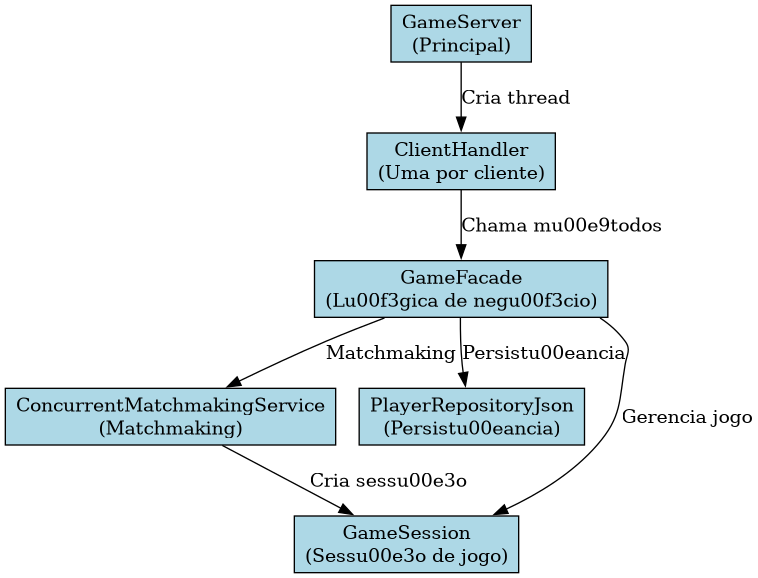
\includegraphics[width=0.9\columnwidth]{figuras/arquitetura.png}
\caption{Diagrama de componentes da arquitetura.}
\label{fig:arquitetura}
\end{figure}

\subsection{Comunicação e API Remota}
A comunicação é realizada por um protocolo textual simples sobre TCP. A Tabela \ref{tab:comandos} descreve os principais comandos da API. O diagrama de sequência na Figura \ref{fig:sequencia} ilustra a interação para o caso de uso de \textit{matchmaking}, desde a requisição do cliente até a criação da sessão de jogo.

\begin{table}[h]
\centering
\caption{Principais comandos da API remota.}
\label{tab:comandos}
\begin{tabular}{@{}ll@{}}
\toprule
Comando & Descrição \\ \midrule
\texttt{CHARACTER\_SETUP} & Configura a raça e classe do personagem. \\ 
\texttt{MATCHMAKING} & Adiciona o jogador à fila de pareamento. \\ 
\texttt{STORE:BUY} & Compra um pacote de cartas na loja. \\ 
\texttt{GAME:PLAY\_CARD} & Executa a jogada de uma carta na partida. \\ 
\texttt{UPGRADE} & Melhora um atributo do jogador. \\ 
\bottomrule
\end{tabular}
\end{table}

\begin{figure}[h]
\centering
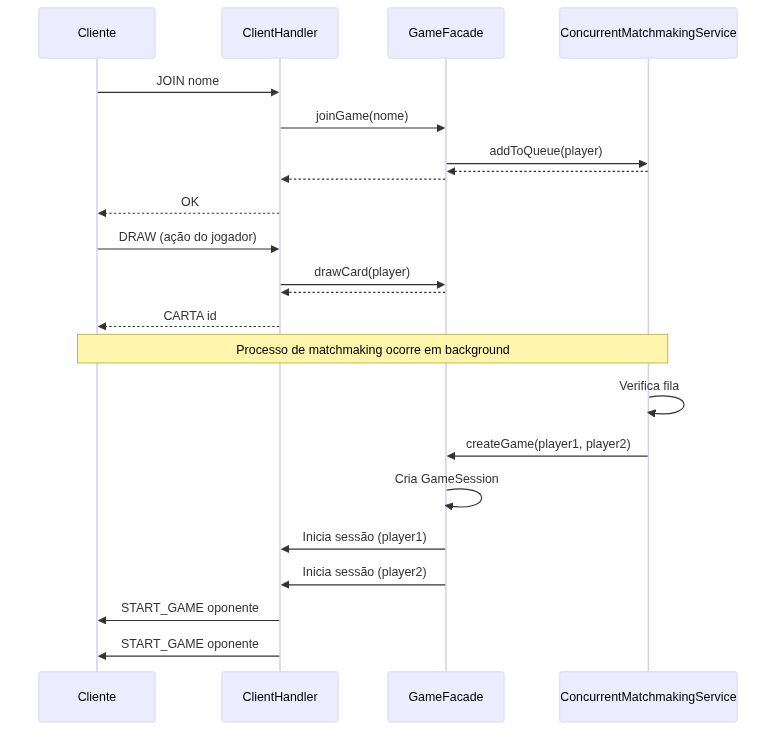
\includegraphics[width=0.9\columnwidth]{figuras/sequencia.png}
\caption{Diagrama de sequência do \textit{matchmaking}.}
\label{fig:sequencia}
\end{figure}

\subsection{Concorrência e Persistência}
Para garantir a segurança em ambiente concorrente, o \texttt{ConcurrentMatchmakingService} utiliza uma \texttt{ConcurrentLinkedQueue} para a fila de jogadores, e o \texttt{GameFacade} gerencia as sessões de jogo e os clientes ativos com \texttt{ConcurrentHashMap}. Essa abordagem minimiza a necessidade de blocos de sincronização explícitos. A persistência é gerenciada pelo \texttt{PlayerRepositoryJson}, que serializa e desserializa os objetos \texttt{Player} de e para arquivos JSON, um para cada jogador.

\subsection{Testes e Emulação}
Uma suíte de testes automatizados foi criada com scripts shell e Docker Compose. O arquivo \texttt{docker-compose.yml} orquestra a criação de um contêiner para o servidor e múltiplos contêineres para os clientes. Os scripts executam cenários específicos para validar a robustez do sistema, como:

\begin{itemize}
    \item \textbf{Desconexão na Fila:} Valida se um jogador que desconecta na fila é removido corretamente e se seu oponente é devolvido à fila.
    \item \textbf{Condição de Corrida:} Simula múltiplas requisições simultâneas para testar a integridade do serviço de \textit{matchmaking}.
    \item \textbf{Malicious Bot:} Envia comandos malformados para garantir que o servidor os rejeite sem comprometer a operação.
    \item \textbf{Teste de Estresse:} Avalia o desempenho e a estabilidade do servidor sob a carga de 10 clientes simultâneos.
\end{itemize}

\section{Resultados}
Os testes automatizados foram cruciais para a validação da arquitetura. A Tabela \ref{tab:resultados} resume os resultados obtidos.

\begin{table}[h]
\centering
\caption{Resumo dos resultados dos testes de cenário.}
\label{tab:resultados}
\begin{tabular}{@{}lp{4.5cm}l@{}}
\toprule
Teste & Objetivo & Resultado \\ \midrule
Desconexão na Fila & Lidar com desconexão de cliente antes do início da partida. & \textbf{Sucesso} \\ \\
Condição de Corrida & Garantir pareamento justo sob múltiplas requisições. & \textbf{Sucesso} \\ \\
Malicious Bot & Validar a robustez contra comandos malformados. & \textbf{Sucesso} \\ \\
Teste de Estresse & Avaliar desempenho com 10 clientes simultâneos por 30s. & \textbf{Sucesso} \\ \\
\bottomrule
\end{tabular}
\end{table}

O teste de "Desconexão na Fila" foi particularmente importante, pois revelou uma condição de corrida no \textit{matchmaking}. A correção, que envolve verificar se ambos os clientes ainda estão ativos \textit{antes} de criar a \texttt{GameSession}, foi validada com sucesso por este teste. O teste de estresse demonstrou que o servidor manteve a estabilidade e a responsividade, processando todas as requisições sem falhas ou perda de dados durante o período de carga.

\section{Conclusão}

Este trabalho demonstrou a implementação bem-sucedida de um servidor de jogo concorrente, o \textit{Dueling Protocol}. A arquitetura, baseada em componentes desacoplados e no uso de padrões de projeto como o \textit{Facade}, provou ser robusta e extensível. O uso de tecnologias padrão de mercado como Java, Sockets, JSON e Docker contribuiu para a criação de uma solução sólida e de fácil manutenção.

A principal contribuição do projeto foi a criação de uma suíte de testes automatizada que não apenas validou os requisitos funcionais, mas também foi fundamental para identificar e corrigir um \textit{bug} de concorrência, ressaltando a importância de testes rigorosos em sistemas distribuídos.

Como trabalhos futuros, vislumbra-se a expansão das mecânicas de jogo, como a implementação de um sistema de energia para as jogadas, a adição de efeitos de cartas mais complexos e a criação de um sistema de montagem de baralhos. A arquitetura base do servidor está preparada para acomodar essas e outras novas funcionalidades.

\bibliographystyle{sbc}
\bibliography{bibliografia}

\end{document}